\documentclass[multi=tikzpicture,border=7pt]{standalone}
\usepackage{ctex,amsmath,bm}
\usepackage{tikz,pgfplots}
\pgfplotsset{compat=1.18}
\usetikzlibrary{arrows.meta,calc,angles,quotes,patterns,positioning,decorations.pathmorphing,3d,intersections}
\tikzset{wire/.style={brown!70!black,very thick},guide/.style={dashed,gray!60},force/.style={->,>=Stealth,thick,red!70!black},velocity/.style={->,>=Stealth,thick,blue!70!black},axis/.style={->,>=Stealth,thick},dim/.style={<->,>=Stealth,thin},body/.style={draw,thick,fill=blue!7},panel/.style={anchor=west,font=\bfseries},hidden/.style={dashed,gray!58,thick},orbit/.style={very thick,blue!70!black}}
\tikzset{charge/.style={circle,draw,fill=blue!12,minimum size=5.5mm,inner sep=0pt},resistor/.style={decorate,decoration={zigzag,segment length=4pt,amplitude=2pt},thick}}
\tikzset{vec/.style={->,>=Stealth,very thick},wall/.style={pattern=north east lines,pattern color=gray},nodept/.style={circle,fill=white,draw,inner sep=1.5pt}}
\begin{document}
% 1 question-01
\begin{tikzpicture}[x=1cm,y=1cm,font=\small]

\node[panel] at (-1.5,2){垂直棱线的截面};\fill[blue!7] (0,0)--(3,1.4)--(3,-1.4)--cycle;\draw[thick] (0,0)--(3,1.4);\draw[thick] (0,0)--(3,-1.4);\draw[guide] (0,0)--(3,0);\fill[orange] (2,0) circle(3pt) node[above]{$Q/L$};\draw[dim] (0,-.3)--(2,-.3) node[midway,below]{$r$};\draw (1.1,-.51) arc(-25:25:1.21);\node[right] at (1.05,.6){$\theta$};\node at (2,-1.8){两边界接地};
\begin{scope}[xshift=6cm]\node[panel] at (-.8,2){沿棱线看长杆};\draw[thick] (0,-1.2)--(0,1.2) node[above]{棱线};\draw[orange,very thick] (2,-1.2)--(2,1.2);\draw[dim] (2.7,-1.2)--(2.7,1.2) node[midway,right]{$L$};\draw[dim] (0,-1.6)--(2,-1.6) node[midway,below]{$r$};\node at (1,-2.3){$L\gg r$};\end{scope}
\end{tikzpicture}

% 2 solution-01
\begin{tikzpicture}[x=1cm,y=1cm,font=\small]

\begin{scope}[xshift=-3.8cm]\node at (0,2.6){$\theta=\pi$};\draw[thick] (0,-2)--(0,2);\fill[blue] (-1.3,0) circle(3pt) node[above]{$-\lambda$};\fill[orange] (1.3,0) circle(3pt) node[above]{$\lambda$};\draw[dim] (-1.3,-.6)--(1.3,-.6) node[midway,below]{$2r$};\draw[force] (1.3,0)--(.5,0);\end{scope}
\begin{scope}[xshift=2.5cm]\node at (0,2.6){$\theta=\pi/10$，含真实线共20个位置};\draw[guide] (0,0) circle(1.9);\fill[blue!9] (0,0)--(2.5,-.396)--(2.5,.396)--cycle;\draw[thick] (0,0)--(2.5,-.396);\draw[thick] (0,0)--(2.5,.396);
\foreach \j in {0,...,19}{\pgfmathsetmacro{\ang}{18*\j}\ifodd\j\fill[blue] (\ang:1.9) circle(2pt);\node[blue,font=\scriptsize] at (\ang:2.12){$-$};\else\fill[red!70!black] (\ang:1.9) circle(2pt);\node[red!70!black,font=\scriptsize] at (\ang:2.12){$+$};\fi}
\draw[force] (1.9,0)--(1.1,0);\node at (.3,-2.8){$\sum_{j=1}^{19}(-1)^j=-1$};\node[right] at (2.3,.65){边界各偏$9^\circ$};\end{scope}
\node at (-.6,-3.5){长杆近似：$F=Q^2/(4\pi\varepsilon_0Lr)$，方向沿平分线向棱线};
\end{tikzpicture}

% 3 question-02
\begin{tikzpicture}[x=1cm,y=1cm,font=\small]
\draw[thick] (0,0)--(1,0);
\draw[thick] (1,0)--(2,0);
\draw[thick] (2,0)--(4,0);
\draw[thick] (4,0)--(5,0);
\draw[thick] (5,0)--(6,0);
\draw[thick] (0,0)--(1,1);
\draw[thick] (1,1)--(2,2);
\draw[thick] (2,2)--(3,3);
\draw[thick] (3,3)--(4,2);
\draw[thick] (4,2)--(5,1);
\draw[thick] (5,1)--(6,0);
\draw[thick] (1,0)--(1,1);
\draw[thick] (2,0)--(2,2);
\draw[thick] (4,0)--(4,2);
\draw[thick] (5,0)--(5,1);
\draw[thick] (1,1)--(2,0);
\draw[thick] (2,2)--(4,0);
\draw[thick] (2,0)--(4,2);
\draw[thick] (4,0)--(5,1);\filldraw[fill=white] (0,0) circle(2pt);
\filldraw[fill=white] (1,0) circle(2pt);
\filldraw[fill=white] (2,0) circle(2pt);
\filldraw[fill=white] (4,0) circle(2pt);
\filldraw[fill=white] (5,0) circle(2pt);
\filldraw[fill=white] (6,0) circle(2pt);
\filldraw[fill=white] (1,1) circle(2pt);
\filldraw[fill=white] (2,2) circle(2pt);
\filldraw[fill=white] (3,3) circle(2pt);
\filldraw[fill=white] (4,2) circle(2pt);
\filldraw[fill=white] (5,1) circle(2pt);
\draw[force] (3,3.8)--(3,3) node[midway,right]{$G$};\draw[force] (1,1.8)--(1,1) node[midway,left]{$P$};\draw[orange,very thick] (2,0)--(4,0) node[midway,below]{目标杆 $N$};\draw[thick] (0,0)--(-.2,-.45)--(.2,-.45)--cycle;\draw[thick] (6,0)--(5.8,-.45)--(6.2,-.45)--cycle;\draw[thick] (-.4,-.5)--(6.4,-.5);\node at (3,-1){交叉斜杆的交点不是铰链};
\end{tikzpicture}

% 4 solution-02
\begin{tikzpicture}[x=1cm,y=1cm,font=\small]
\draw[gray] (0,0)--(1,0);
\draw[gray] (1,0)--(2,0);
\draw[gray] (2,0)--(4,0);
\draw[gray] (4,0)--(5,0);
\draw[gray] (5,0)--(6,0);
\draw[gray] (0,0)--(1,1);
\draw[gray] (1,1)--(2,2);
\draw[gray] (2,2)--(3,3);
\draw[gray] (3,3)--(4,2);
\draw[gray] (4,2)--(5,1);
\draw[gray] (5,1)--(6,0);
\draw[gray] (1,0)--(1,1);
\draw[gray] (2,0)--(2,2);
\draw[gray] (4,0)--(4,2);
\draw[gray] (5,0)--(5,1);
\draw[gray] (1,1)--(2,0);
\draw[gray] (2,2)--(4,0);
\draw[gray] (2,0)--(4,2);
\draw[gray] (4,0)--(5,1);\filldraw[fill=white] (0,0) circle(2pt);
\filldraw[fill=white] (1,0) circle(2pt);
\filldraw[fill=white] (2,0) circle(2pt);
\filldraw[fill=white] (4,0) circle(2pt);
\filldraw[fill=white] (5,0) circle(2pt);
\filldraw[fill=white] (6,0) circle(2pt);
\filldraw[fill=white] (1,1) circle(2pt);
\filldraw[fill=white] (2,2) circle(2pt);
\filldraw[fill=white] (3,3) circle(2pt);
\filldraw[fill=white] (4,2) circle(2pt);
\filldraw[fill=white] (5,1) circle(2pt);
\draw[force] (2,0)--(2.75,0) node[above]{$N$};\draw[force] (4,0)--(3.25,0) node[above]{$N$};\draw[velocity] (1,1)--(1.3,.5) node[left]{$\delta h_P=-\delta x/2$};\draw[velocity] (3,3)--(3.3,2.5) node[right]{$\delta h_G=-\delta x/2$};\draw[velocity] (6,0)--(6.8,0) node[above]{$\delta x_f=\delta x$};\draw[dim] (2,-.55)--(4,-.55) node[midway,below]{$\delta x>0$};\node at (3,-1.4){切杆两端拉力向内：虚功 $-N\delta x$};\node at (3,-2.1){$N=(G+P)/2+f$，$|f|\leq\mu(G/2+P/6)$};
\end{tikzpicture}

% 5 question-03
\begin{tikzpicture}[x=1cm,y=1cm,font=\small]

\draw[body] (-3,0) rectangle(3,.6);\draw[dim] (-3.4,0)--(-3.4,.6) node[midway,left]{$l$};\foreach \x in {-1,1}{\draw[thick] (\x,-.45) circle(.45);\draw[body] (\x-.13,.6) rectangle(\x+.13,1.3);}\draw[velocity] (-1.2,-.9) arc(-115:-375:.49);\draw[velocity] (1.2,-.9) arc(-65:195:.49);\draw[dim] (-1,-1.2)--(1,-1.2) node[midway,below]{$2l$};\fill (0,.3) circle(2pt);\draw[velocity] (0,.3)--(.9,.3) node[above]{$v_0$};\node at (0,1.8){固定上柱与板初始虚接触；滚筒顶部向中间运动};
\end{tikzpicture}

% 6 solution-03
\begin{tikzpicture}[x=1cm,y=1cm,font=\small]

\foreach \shift/\txt in {0/{向右外行：$\dot x>0$},5.5/{向左返回：$\dot x<0$}}{\begin{scope}[xshift=\shift cm]
\node at (0,2){\txt};\draw[body] (-1.7,0) rectangle(2,.6);\draw[force] (-1,.6)--(-1,-.2) node[left]{$N_1$};\draw[force] (1,0)--(1,.8) node[right]{$N_2$};\draw[force] (1,0)--(.3,0) node[below]{$\mu N_2$};\end{scope}}
\draw[force] (-1,.6)--(-1.7,.6) node[above]{$\mu N_1$};\draw[force] (4.5,.6)--(5.2,.6) node[above]{$\mu N_1$};\node at (0,-1){$a=-g(x+l/4)/(2l)$};\node at (5.5,-1){$a=-g/2$};
\begin{scope}[yshift=-3.6cm]\draw[axis] (0,0)--(4.3,0) node[right]{$x/l$};\draw[axis] (0,0)--(0,1.8) node[above left]{$-a/g$};\draw[blue,thick] (0,0)--(2.25,1.125);\draw[blue,thick] (2.25,1.125)--(3,1.40625);\draw[orange,thick] (2.25,1.125)--(3,1.125);\draw[guide] (2.25,0)--(2.25,1.8);\node[below] at (2.25,0){$3/4$};\node[below] at (3,0){$1$};\node[blue] at (4,1.6){外行};\node[orange] at (4,.9){返回};\node[align=left] at (7,.9){中央区 $a=-2gx/(3l)$\\$\delta'=\sqrt{l^2+2l\delta}-l$\\长期 $u_2=\sqrt{3gl/8}$};\end{scope}
\end{tikzpicture}

% 7 question-04
\begin{tikzpicture}[x=1cm,y=1cm,font=\small]

\begin{scope}\node at (1,3.6){导轨平面内俯视};\draw[wire] (0,0)--(0,3);\draw[wire] (2,0)--(2,3);\draw[wire] (0,0)--(2,0);\draw[orange,very thick] (0,1.7)--(2,1.7);\draw[dim] (0,-.45)--(2,-.45) node[midway,below]{$l$};\draw[dim] (2.5,0)--(2.5,1.7) node[midway,right]{$x_0$};\draw[velocity] (1,1.7)--(1,2.6) node[right]{$I_0$};\end{scope}
\begin{scope}[xshift=5cm]\node at (1,3.6){侧视：倾角 $\theta$};\draw[thick] (0,0)--(3.46,2);\draw[guide] (0,0)--(3.8,0);\draw (1,0) arc(0:30:1);\node at (1.3,.3){$\theta$};\filldraw[fill=orange] (2.1,1.21) circle(3pt);\draw[force] (2.1,1.21)--(2.1,.2) node[right]{$mg$};\draw[velocity] (2.1,2.9)--(2.1,2) node[right]{$\boldsymbol B$};\draw[dim] (.3,-.4)--(2.4,.81) node[midway,below]{$x$};\end{scope}
\end{tikzpicture}

% 8 solution-04
\begin{tikzpicture}[x=1cm,y=1cm,font=\small]

\draw[axis] (0,0)--(4.6,0) node[below right]{$y$};\draw[axis] (0,0)--(0,3.3) node[above]{$U_{\rm eff}/(mgx_0)$};\draw[orbit,domain=.28:2.2,samples=120] plot({2*\x},{2*\x-3+1.5/\x});\draw[orange,thick] (.5,1.75)--(4.2,1.75);\fill[orange] (.75,1.75) circle(2pt);\fill[orange] (4,1.75) circle(2pt);\draw[guide] (.75,0)--(.75,1.75);\draw[guide] (4,0)--(4,3.1);\node[below] at (.75,0){$3/8$};\node[below] at (2,0){$1$};\node[below] at (4,0){$2$};\node[orange] at (2.5,2){临界能量 $7/4$};
\node[draw,align=left] at (7.3,1.3){$i=(Bl\cos\theta/k)(1-1/y)$\\[5pt]$N/(mg\cos\theta)=2/y-1$\\[5pt]$F_x=-mg\sin\theta-ai+ki^2/2$\\[5pt]$a=Bl\cos\theta$,\quad $y=x/x_0$};\node at (4,-1){上行转折与 $N=0$ 在 $y=2$ 重合；自感梯度力必须保留};
\end{tikzpicture}

% 9 question-05
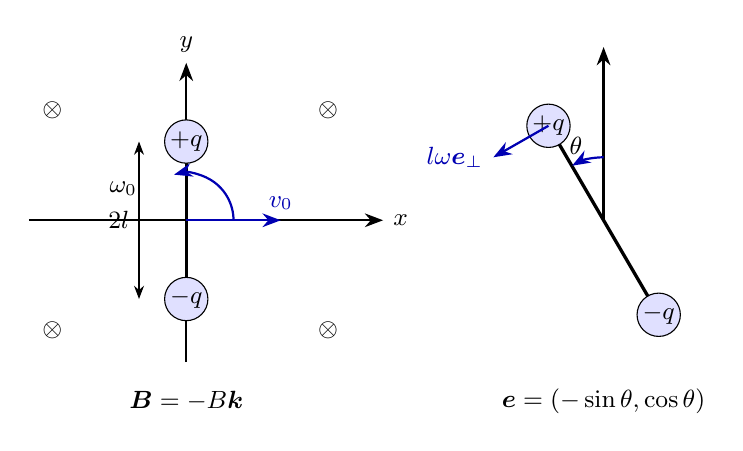
\begin{tikzpicture}[x=1cm,y=1cm,font=\small]

\draw[axis] (-2,0)--(2.5,0) node[right]{$x$};\draw[axis] (0,-1.8)--(0,2) node[above]{$y$};\draw[very thick] (0,-1)--(0,1);\node[charge] at (0,1){$+q$};\node[charge] at (0,-1){$-q$};\draw[velocity] (0,0)--(1.2,0) node[above]{$v_0$};\draw[velocity] (.6,0) arc(0:105:.6);\node at (-.8,.4){$\omega_0$};\draw[dim] (-.6,-1)--(-.6,1) node[midway,left]{$2l$};\foreach \p in {(-1.7,1.4),(1.8,1.4),(-1.7,-1.4),(1.8,-1.4)}{\node at \p{$\otimes$};}\node at (0,-2.3){$\boldsymbol B=-B\boldsymbol k$};
\begin{scope}[xshift=5.3cm]\draw[axis] (0,0)--(0,2.2);\draw[very thick] (.7,-1.2)--(-.7,1.2);\node[charge] at (-.7,1.2){$+q$};\node[charge] at (.7,-1.2){$-q$};\draw[velocity] (0,.8) arc(90:120:.8);\node at (-.35,.95){$\theta$};\draw[velocity] (-.7,1.2)--(-1.4,.8) node[left]{$l\omega\boldsymbol e_\perp$};\node at (0,-2.3){$\boldsymbol e=(-\sin\theta,\cos\theta)$};\end{scope}
\end{tikzpicture}

% 10 solution-05
\begin{tikzpicture}[x=1cm,y=1cm,font=\small]

\draw[axis] (-1.5,0)--(1.5,0) node[below right]{$v_x-v_0-K$};\draw[axis] (0,-1.5)--(0,1.5) node[above]{$v_y$};\draw[orbit] (0,0) circle(1);\fill (1,0) circle(2pt);\fill (-1,0) circle(2pt);\node[above right] at (1,0){$\theta=\pi$};\node[above left] at (-1,0){$\theta=0$};\draw[velocity] (-1,0) arc(180:260:1);\node at (0,-2){速度圆：半径 $K$};
\begin{scope}[xshift=5cm]\draw[thick] (-.6,1)--(3.5,1);\draw[thick] (-.6,-2.15)--(3.5,-2.15);\draw[orange,very thick] (0,-1)--(0,1);\draw[orange,very thick] (2,-2.15)--(2,-.15);\fill (0,0) circle(2pt);\fill (2,-1.15) circle(2pt);\draw[dim] (3,1)--(3,-2.15) node[midway,right]{$\Delta h$};\node at (1.4,1.6){转动：最低点在 $\theta=\pi$};\node[align=center] at (1.5,-3){$\Delta h/l=2+(s_0-\sqrt{s_0^2-4KA})/A$};\end{scope}
\node[draw,align=left] at (4,-4.5){摆动：返回到 $\theta=0,\ s=-s_0$ 给出最低点\\$\Delta h/l=2+2s_0/A$\\临界轨道：只到 $s\to0$，不进入返回支路};
\end{tikzpicture}

% 11 question-06
\begin{tikzpicture}[x=1cm,y=1cm,font=\small]

\draw[thick] (0,0)--(7,0);\draw[thick] (0,1.5)--(7,1.5);\draw[thick] (0,0)--(0,1.5);\draw[fill=orange!25,thick] (2,0) rectangle(2.4,1.5);\fill[blue!10] (.03,.03) rectangle(1.98,1.47);\node at (1,.8){$P_0,V_0$};\node at (4.6,.8){$P_{\rm atm}$};\draw[velocity] (2.5,1.8)--(3.7,1.8) node[above]{土豆};\draw[dim] (0,-.6)--(7,-.6) node[midway,below]{总长度 $L$};\draw[dim] (0,2.2)--(2,2.2) node[midway,above]{$V_0/A$};\node[right] at (7,.8){开口};\node at (3.5,-1.5){出管体积 $V=AL$；土豆行程 $s=L-V_0/A$};
\end{tikzpicture}

% 12 solution-06
\begin{tikzpicture}[x=1cm,y=1cm,font=\small]

\draw[axis] (0,0)--(6,0) node[right]{$V/V_0$};\draw[axis] (0,0)--(0,4.5) node[above]{$P/P_{\rm atm}$};\fill[blue!15] (1,1)--plot[domain=1:2.6918,samples=90] (\x,{4*pow(\x,-1.4)})--(2.6918,1)--cycle;\draw[orbit,domain=1:5,samples=100] plot(\x,{4*pow(\x,-1.4)});\draw[orange,thick] (.7,1)--(5.4,1);\draw[guide] (2.6918,0)--(2.6918,2.3);\node[below] at (1,0){$1$};\node[below] at (2.6918,0){$V_*/V_0$};\node at (2,2.4){正面积为净功};\node[align=left] at (8,2){$P(V_*)=P_{\rm atm}$\\[6pt]$V_*=V_0(P_0/P_{\rm atm})^{5/7}$\\[6pt]$L_*=V_*/A$};\node at (3,-1){示例 $P_0/P_{\rm atm}=4$；交点之后新增面积为负};
\end{tikzpicture}

% 13 question-07
\begin{tikzpicture}[x=1cm,y=1cm,font=\small]

\draw[axis] (-2.5,0)--(5.8,0);\fill ( -2,0) circle(2pt) node[above]{光源};\draw[blue,very thick] (0,.18)--(0,1.3);\draw[blue,very thick] (0,-.18)--(0,-1.3);\fill[black] (-.07,-.18) rectangle(.07,.18);\draw[dim] (.5,-.18)--(.5,.18) node[right]{$\delta$};\draw[thick] (5,-1.5)--(5,1.5) node[above]{屏};\draw[dim] (-2,-1.9)--(0,-1.9) node[midway,below]{$p$};\draw[dim] (0,-1.9)--(5,-1.9) node[midway,below]{$H$};\node at (1.5,2){上下半片的局部光轴间距为 $\delta$};
\end{tikzpicture}

% 14 solution-07
\begin{tikzpicture}[x=1cm,y=1cm,font=\small]

\draw[axis] (-2.4,0)--(5.7,0);\fill (-2,0) circle(2pt) node[above]{$S$};\draw[blue,very thick] (0,.18)--(0,1.4);\draw[blue,very thick] (0,-.18)--(0,-1.4);\fill (-.06,-.18) rectangle(.06,.18);\draw[thick] (5,-1.7)--(5,1.7);
\draw[orange,thick] (-2,0)--(0,.18)--(2,.36)--(5,.63);\draw[orange,thick] (-2,0)--(0,1.4)--(2,.36)--(5,-1.2);\draw[blue,thick] (-2,0)--(0,-.18)--(2,-.36)--(5,-.63);\draw[blue,thick] (-2,0)--(0,-1.4)--(2,-.36)--(5,1.2);\fill[orange] (2,.36) circle(2pt) node[above]{$S_1$};\fill[blue] (2,-.36) circle(2pt) node[below]{$S_2$};\draw[dim] (2.5,-.36)--(2.5,.36) node[right]{$d$};\draw[orange,very thick] (5,-.63)--(5,.63);\draw[dim] (5.45,-.63)--(5.45,.63) node[right]{$D$};\draw[dim] (0,-2.1)--(2,-2.1) node[midway,below]{$q$};\draw[dim] (2,-2.1)--(5,-2.1) node[midway,below]{$h=H-q$};\node at (1.5,2){内边缘光线在各自半片光轴上不偏折};\node at (1.5,-3){$\Delta=\lambda h/d$；$|n|\leq23.33$，共47条亮纹};
\end{tikzpicture}

% 15 question-08
\begin{tikzpicture}[x=1cm,y=1cm,font=\small]

\draw[body] (0,0) rectangle(1.4,1);\node at (.7,.5){激光};\draw[velocity] (1.6,.5)--(3,.5) node[above]{光束};\node[charge] at (3.7,.5){$+$};\draw[velocity] (3.4,.2)--(2.6,.2) node[below]{$v$};\draw[body] (5.1,0) rectangle(6.7,1);\node at (5.9,.5){探测器};\draw[force] (3.9,.7)--(5.05,.7) node[above]{荧光};\draw[axis] (7.8,0)--(10.8,0) node[right]{$v$};\draw[axis] (7.8,0)--(7.8,1.8) node[above]{$dN/dv$};\draw[thick] (7.8,1.1)--(10,1.1)--(10,0);\node[below] at (7.8,0){$0$};\node[below] at (10,0){$5000$};\node at (5,-1.2){离子朝光源运动，实验室共振波长比静止值长};
\end{tikzpicture}

% 16 solution-08
\begin{tikzpicture}[x=1cm,y=1cm,font=\small]

\draw[axis] (0,0)--(5.7,0);\node at (2.2,-.6){$\lambda-580\ \mathrm{nm}$};\draw[axis] (0,0)--(0,2) node[above]{$dN/d\lambda$};\draw[blue,thick] (0,1.3)--(4.35,1.3)--(4.35,0);\node[below] at (0,0){$0$};\node[below] at (4.35,0){$0.00967$};\node at (2.4,2.5){矩形分布的线性映射};\node at (2.5,-1){未加速，两扫描段重叠};
\draw[blue,very thick] (0,-2)--(4.35,-2);\draw[orange,very thick] (.45,-2.6)--(4.8,-2.6);\node[left] at (0,-2){$\lambda_1$};\node[left] at (.45,-2.6){$\lambda_2$};
\node at (8,2.5){预加速：两扫描区间端点相切};\node at (8,2.05){横线表示范围，非谱形};\draw[axis] (6,0)--(11.2,0);\draw[blue,very thick] (6.3,.7)--(8.3,.7);\draw[orange,very thick] (8.3,1.4)--(10.3,1.4);\draw[guide] (8.3,0)--(8.3,1.8);\node[below] at (8.3,-.4){$\lambda_1(1+u_2/c)=\lambda_2(1+s/c)$};\node[align=center] at (8.5,-2){$s=\sqrt{2(q/m)V}$\\$u_2=\sqrt{s^2+v_2^2}$\\$V_{\rm crit}\simeq57.2\ \mathrm V$};
\end{tikzpicture}

\end{document}
